%\documentclass[english,10pt,handout]{beamer}
\documentclass[english,10pt]{beamer}







 
%\usepackage{mathptmx}
%\renewcommand{\sfdefault}{lmss}
\usepackage[T1]{fontenc}
%\usepackage[latin9]{inputenc}
\usepackage[utf8]{inputenc}

\synctex=-1

\usefonttheme{professionalfonts}

%\setbeamertemplate{navigation symbols}{}
%\setbeamertemplate{caption}[numbered]


\useinnertheme{rectangles}
%http://tex.stackexchange.com/questions/11168/change-bullet-style-formatting-in-beamer

 \AtBeginDocument{
  \addtolength\abovedisplayskip{-0.4\baselineskip}%
  \addtolength\belowdisplayskip{-0.4\baselineskip}%
}%change the space between text lines and the math formula


\usepackage{pifont}
%Postscript ZipfDingbats font
%the command \ding{number}, will print the specified symbol

\usepackage{fontawesome}
%icon package
\DeclareFontFamily{U}{FontAwesomeOne}{}
\DeclareFontShape{U}{FontAwesomeOne}{m}{n}{<-> FontAwesome--fontawesomeone}{}
\DeclareRobustCommand\FAone{\fontencoding{U}\fontfamily{FontAwesomeOne}\fontseries{m}\fontshape{n}\selectfont}
\DeclareFontFamily{U}{FontAwesomeTwo}{}
\DeclareFontShape{U}{FontAwesomeTwo}{m}{n}{<-> FontAwesome--fontawesometwo}{}
\DeclareRobustCommand\FAtwo{\fontencoding{U}\fontfamily{FontAwesomeTwo}\fontseries{m}\fontshape{n}\selectfont}
\DeclareFontFamily{U}{FontAwesomeThree}{}
\DeclareFontShape{U}{FontAwesomeThree}{m}{n}{<-> FontAwesome--fontawesomethree}{}
\DeclareRobustCommand\FAthree{\fontencoding{U}\fontfamily{FontAwesomeThree}\fontseries{m}\fontshape{n}\selectfont}

%ftp://ftp.dante.de/tex-archive/fonts/fontawesome/doc/fontawesome.pdf
%http://tug.ctan.org/info/symbols/comprehensive/symbols-a4.pdf


\usepackage{amsmath,amssymb,amsfonts,bm,mathrsfs,mathtools}

\usepackage{tikzsymbols}
%\usepackage[tikz]{bclogo}



\usepackage{perpage}
\MakePerPage{footnote} %reset for each page
%\renewcommand{\thefootnote}{\fnsymbol{footnote}} %use symbol, limit less than 9 symbols



%%%% HIGHTLIGHT  and annotation &=%%%%%%%%
\usepackage{color,xcolor}
 \usepackage{todonotes}

\usepackage[normalem]{ulem}

\usepackage[many]{tcolorbox}

\tcbset{fonttitle=\scriptsize}
\tcbset{highlight math style={enhanced,
  colframe=red!40!black,colback=yellow!20!white,arc=2pt,boxrule=.2pt,
  }}
  \newtcbox{\otherbox}[1][]{nobeforeafter,math upper,tcbox raise base,
enhanced,frame hidden,boxrule=0pt,interior style={top color=green!10!white,
bottom color=green!10!white,middle color=green!50!yellow},
fuzzy halo=1pt with green,#1}
%%\tcbhighmath{math here}
%% \otherbox{math here}



%%%%% HIGHLIGHT %%%%%%
\newcommand{\hb}[1]{{\color{blue}{#1}}}
%\noindent\rule{\textwidth}{.5pt}

%:
\usepackage{soul}

\newcommand\hcancel[2][black]{\setbox0=\hbox{$#2$}%
\rlap{\raisebox{.45\ht0}{\textcolor{#1}{\rule{\wd0}{1pt}}}}#2}
%cross to delete

\newcommand{\mcb}[2]{\colorbox{#1}{$\displaystyle #2$}}
%highlight math

\newcommand{\hlfancy}[2]{\sethlcolor{#1}\hl{#2}}
%specified color , for\hl

\newcommand\myhl{\bgroup\markoverwith
  {\textcolor{yellow}{\rule[-.5ex]{2pt}{2.5ex}}}\ULon}



\mode<presentation>{ \usetheme{boxes} }

%write Matlab code
\usepackage{listings}
 \definecolor{dkgreen}{rgb}{0,0.6,0}
\definecolor{gray}{rgb}{0.5,0.5,0.5}
\definecolor{mauve}{rgb}{0.58,0,0.82}
\lstset{frame=tb,
  language=Matlab,
  aboveskip=3mm,
  belowskip=3mm,
  showstringspaces=false,
  columns=flexible,
  basicstyle={\small\ttfamily},
  numbers=none,
  numberstyle=\tiny\color{gray},
  keywordstyle=\color{blue},
  commentstyle=\color{dkgreen},
  stringstyle=\color{mauve},
  breaklines=true,
  breakatwhitespace=true
  tabsize=3
}

\usepackage[lastexercise]{exercise}

\newtheorem{ex}{Exercise}
\newtheorem{property}{Property}
\newtheorem{ag}{Algorithm}
\newtheorem{remark}{Remark}
\newtheorem{den}{definition}
\newtheorem{assumption}{Assumption}


\usepackage[nosolutionfiles]{answers}
\Newassociation{sol}{Solution}{ans}



\usepackage{empheq}
\usepackage{comment}
%\usepackage{lscape}
\usepackage{multirow}
\usepackage{url,hyperref}

\hypersetup{
 %   bookmarks=true,         % show bookmarks bar?
    unicode=false,          % non-Latin characters in Acrobat's bookmarks
    pdftoolbar=true,        % show Acrobat's toolbar?
    pdfmenubar=true,        % show Acrobat's menu?
    pdffitwindow=false,     % window fit to page when opened
    pdfstartview={FitH},    % fits the width of the page to the window
    pdftitle={My title},    % title
    pdfauthor={Author},     % author
    pdfsubject={Subject},   % subject of the document
    pdfcreator={Creator},   % creator of the document
    pdfproducer={Producer}, % producer of the document
    pdfkeywords={keyword1} {key2} {key3}, % list of keywords
    pdfnewwindow=true,      % links in new window
    colorlinks=true,       % false: boxed links; true: colored links
    linkcolor=red,          % color of internal links (change box color with linkbordercolor)
    citecolor=green,        % color of links to bibliography
    filecolor=magenta,      % color of file links
    urlcolor=cyan           % color of external links
}


\usepackage{subfigure,epsfig,graphicx,graphics}

\DeclareGraphicsRule{.tif}{png}{.png}{`convert #1 `dirname #1`/`basename #1 .tif`.png}
   \DeclareGraphicsExtensions{.pdf}




\newcommand{\hw}{ {\underline{\tt Homework }} }
\newcommand{\hws}{ {\underline{\tt Homework$\star$}} }
\newcommand{\optional}{ {\it optional} }

\newcommand{\MATLAB}{ \texttt{MATLAB}}
\newcommand{\python}{ \texttt{python}}
\newcommand{\Rlang}{ \texttt{R}}
\newcommand{\SAS}{ \texttt{SAS}}
\newcommand{\MC}{Markov Chain}


\newcommand{\tm}{transition matrix}
\newcommand{\rv}{random variable}
\newcommand{\spl} {supervised learning }
 

\newcommand{\dis}{\underline{\tt discussion}: }
\newcommand{\pri}{\underline{\tt principle}: }




\newcommand{\bq}{\scalebox{6}{\textbf{?} }}
\newcommand{\sq}{\scalebox{2}{\textbf{?} }}
\newcommand{\ck} {  {\scalebox{0.8} {\Interval}   } }

\newcommand{\eps}{\varepsilon}
\newcommand{\To}{\longrightarrow}

% 
\newcommand{\Dcal}{\mathtt{D}}
\newcommand{\Hcal}{\mathcal{H}}
\newcommand{\Ecal}{\mathcal{E}}
\newcommand{\Xcal}{\mathcal{X}}
\newcommand{\Ycal}{\mathcal{Y}}
\newcommand{\Zcal}{\mathcal{Z}}

%%Calculus 

\renewcommand{\d}{\ensuremath{\mathrm{d}}}
\newcommand{\dt}{ \ensuremath{\mathrm{d} t } }
\newcommand{\dx}{ \ensuremath{\mathrm{d} x} }
\newcommand{\dy}{ \ensuremath{\mathrm{d} y } }

%indicator function
\newcommand{\indf}{ \ensuremath{\mathbf{1} } }



%probability
\newcommand{\p}{ \mathbb{P}}
\newcommand{\prob}{{\Pr}}
\newcommand{\PP}{\mbox{PP}}%Poisson process
%condition prob
\newcommand{\cPr}[2]{{\Pr\left(#1\mid #2\right)}}

\newcommand{\FF}{{\mathbb{F}}}

\newcommand{\e}{ \operatorname{\mathbb E}}
\newcommand{\Var}{\operatorname{\mathbb{V} }}
\newcommand{\var}{\operatorname{\text{Var} }}
\newcommand{\MSE}{\operatorname{\text{MSE} }}

\newcommand{\Std}{\operatorname{std}}
\newcommand{\Cov}{\operatorname{cov}}

%Matrix  %mathbf
\newcommand{\Pb}{{\mathbf{P}}}
\newcommand{\Qb}{{\mathbf{Q}}}
\newcommand{\Mb}{{\mathbf{M}}}
\newcommand{\cb}{\mathbf{c}}
\newcommand{\bb}{{\mathbf{b}}}

\newcommand{\Tb}{\mathbf{T}}

\newcommand{\Wb}{\mathbf{W}}
\newcommand{\wb}{\mathbf{w}}
\newcommand{\Xb}{\mathbf{X}}

\newcommand{\xb}{\mathbf{x}}

\newcommand{\Wtn}{\mathbb{W}}
\newcommand{\btn}{\mathbf{b}}



\newcommand{\eye}{{\mathbf{I}}}
%identity matrix
\newcommand{\onem}{{\mathbb{1}}}
\newcommand{\idor}{\mathbf{1}}
\newcommand{\ii}{\mathbf{i}}
%imaginary symbol

\usepackage{tikz}

%State number
\newcommand{\snum}[1]{ \raisebox{.5pt}{\textcircled{\raisebox{-.9pt} {#1}}}}

 \usetikzlibrary{arrows}
\usetikzlibrary{shapes}

%\newcommand{\snum}[1]{%
 % \tikz[baseline=(char.base)]\node[anchor=south west, draw,rectangle, rounded corners, inner sep=1.4pt, minimum size=5mm,
   % text height=1.3mm](char){\ensuremath{#1}} ;}

\newcommand*\circled[1]{\tikz[baseline=(char.base)]{
            \node[shape=circle,draw,inner sep=.4pt] (char) {#1};}}


%real number
\newcommand{\Real}{{\mathbb{R}}}
%integer
\newcommand{\ZZ}{\mathbb{Z}}
%positive integer
\newcommand{\NN}{\mathbb{N}}



\newcommand{\inpd}[2]{\left\langle #1, #2 \right\rangle}
\newcommand{\abs}[1]{\left\vert#1\right\vert}
\newcommand{\norm}[1]{\left\|#1\right\|}
\newcommand{\wt}[1]{{\widetilde{#1}}}
\newcommand{\set}[1]{\left\{#1\right\}}
\newcommand{\partiald}[2]{  \frac{\partial #1 }{\partial #2}}



\newcommand{\ie}{{\it{i.e.}}}



\newcommand{\transpose}{\textsf{T}} % or, \intercal
\newcommand{\diag}{\textsf{diag}}
\newcommand{\tr}{{\textsf{T}}}
\newcommand{\rt}{{\textbf{r}}}

\DeclareMathOperator{\trace}{Trace}


\newcommand{\argmin}{ \operatornamewithlimits{argmin} }
\newcommand{\argmax}{ \operatornamewithlimits{argmax} }




\def\biz{\begin{itemize} }
\def\bizp{\begin{itemize}[<+->] }
\def\eiz{\end{itemize}}


\def\bfm{\begin{frame}}
\def\efm{\end{frame}}

\def\bena{\begin{enumerate}[<+-| alert@+>]}
\def\ben{\begin{enumerate}}
\def\een{\end{enumerate}}


\def\bbk{\begin{block} }
\def\ebk{\end{block}}






\makeatletter
%%%%%%%%%%%%%%%%%%%%%%%%%%%%%% Textclass specific LaTeX commands.
 % this default might be overridden by plain title style

%%%%%%%%%%%%%%%%%%%%%%%%%%%%%% User specified LaTeX commands.
%\usetheme{Warsaw}
\usetheme{Boadilla}
% or ...



%\setbeamertemplate{footline}[text line]{} % makes the footer EMPTY
%\setbeamertemplate{footline}[page number]{} % makes the footer EMPTY

%\usecolortheme{orchid} %not use is better 

\setbeamertemplate{footline}[text line]{%
  \parbox{\linewidth}{\vspace*{-2pt}Xiang Zhou\hfill CityU\hfill \insertpagenumber}}
%\setbeamertemplate{navigation symbols}{}

%\setbeamercovered{transparent}
% or whatever (possibly just delete it)


%\usepackage{babel}
\makeatother



 %
%\addtobeamertemplate{frametitle}{}{%
%\begin{tikzpicture}[remember picture,overlay]
%\node[anchor=south east,yshift=2pt] at (current page.south east) {
\includegraphics[height=0.6cm]{CityU_Logo_Basic_Signature.eps}};
%\end{tikzpicture}}
%

\beamerdefaultoverlayspecification{<+->}
%the presentation acts as though a \pause command has been inserted between every two bullets, without the actual need to write \pause after each item.




\begin{document}





\title{Introduction to Stochastic Process}


\author{Xiang Zhou}


%\date[CFP 2003]{2013-2014, Semester A}


 

\frame{{Chapter 2: Discrete-Time Markov Models (Part i)}
\begin{center}

\includegraphics[scale=0.4]{Markov-chain-banner.png}
\bigskip \par 
 Andrey  Markov (1856-1922, Russian mathematician)
\end{center}
}

\frame{
\frametitle{life is a \emph {game} with  uncertainty: }
\begin{center}
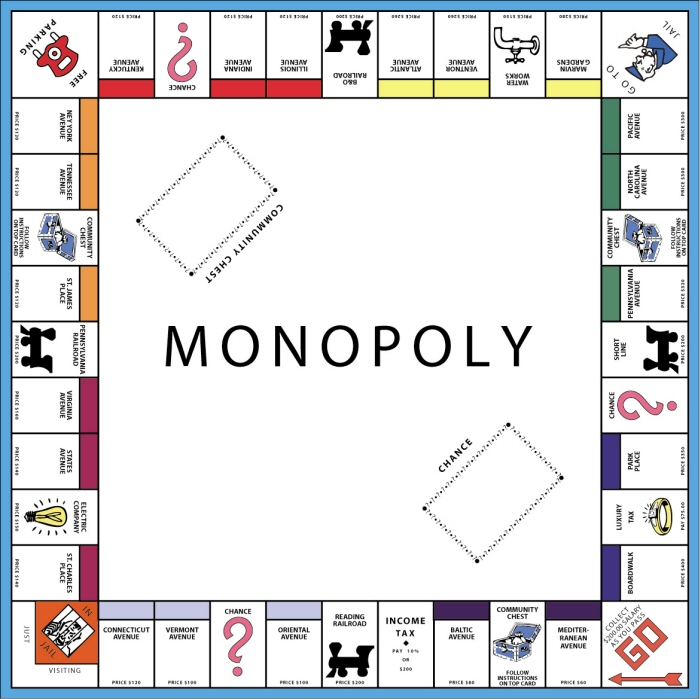
\includegraphics[width=0.6\textwidth]{Monopoly-700x699.jpg}
\\
Game of Monopoly: at least 40 states where you live in
\end{center}}



\frame{
\begin{center}

\includegraphics[width=0.6\textwidth]{Monopoly-with-dice-paths.png}
\\
At least 40 $\times$ 11 transitions between states.
\end{center}
}

\frame{
\begin{center}

\includegraphics[width=0.6\textwidth]
{Monopoly-with-dice-paths-from-jail.png}\\
\biz
\item { Fate (next state) depends on where you are (current state ).}
\item { Fate does {\it  not } depend on how you got there (history).}
\eiz
\end{center}
}



\frame{
\frametitle{What we learn from 
Game of Monopoly}

\bigskip
\pause 
\begin{center}
\tt{
 \uppercase{  Yesterday is history. Tomorrow is a mystery. 
 \\ Today is a gift.} 
 }
\end{center}

\pause
\hspace{5cm}-- \footnotesize{  the Turtle ( {\it Kung Fu Panda (movie) } )}

\bigskip
\pause

{\bf Markovian property: }
\biz
\item 
$X_{n+1} $ is a random variable, whose \underline{law} (distribution) is determined only by the \underline{current value} of $X_n$ and independent of all   history $X_{n-1}, X_{n-2}, \cdots$.
\item 
The law governing the distribution of $X_{n+1}$ (given the value of $X_n$) is called  \emph{transition probability}:  $\p(X_{n+1}=?\vert X_n)$ 
\eiz

\pause
Corollary: 
\biz 
\item  What is the joint distribution of $(X_{n+1}, X_n)$ ? 
   $\p(X_{n+1}, X_n) = \p(X_{n+1}|X_n)\p(X_n)$
\item What is the (marginal) distribution of $X_{n+1}$ ? 
   $\p(X_{n+1}) = \sum_x \p(X_{n+1}, X_n=x)  = \sum_x \p(X_{n+1}\vert X_n=x)\p(X_n=x)$

 \eiz 



}





\frame{
 { Markov model of the weather }
 \begin{figure}
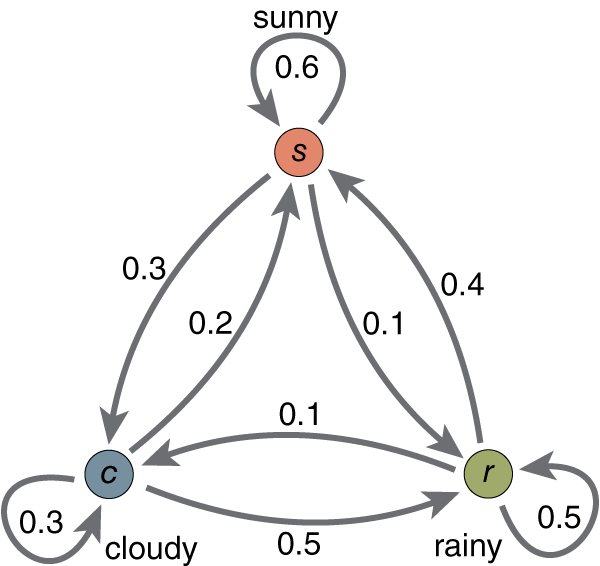
\includegraphics[width=0.46\textwidth]{weather-model.png}
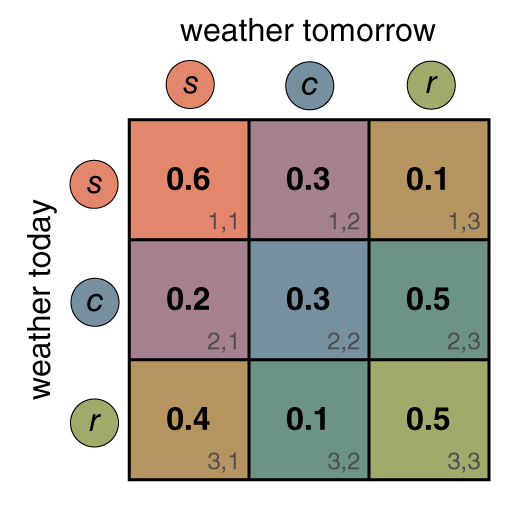
\includegraphics[width=0.46\textwidth]{weather-matrix.png}
\caption{transition diagram and transition matrix}
\end{figure}
}

\begin{frame}
\frametitle{Theory of DTMC}
\begin{definition}%{}
A stochastic process $\{X_{n},n\geq0\}$ on state space $S$ is said
to be a discrete-time Markov chain (DTMC) if ,  for all $i$ and
$j$ in $S$ ,
\[
\p(X_{n+1}=j\:\vert X_{n}=i,\, X_{n-1},\ldots X_{0})=\p(X_{n+1}=j\:\vert X_{n}=i)
\]


A DTMC $\{X_{n}\}$ is said to be \textit{time-homogeneous} if, for
all $n=0,1,2,\ldots$,
\[
\p(X_{n+1}=j\:\vert X_{n}=i)
\]
is {\it independent}  of the time $n$.
\end{definition}%{}
In this chapter we mainly  consider   time-homogeneous DTMCs with
finite state space $S=\{1,2,3,\cdots,N\}$, and  occasionally  
we may consider  state space with countable infinite elements labelled as  $S=\mathbb{N}:=\{1,2,3,\cdots\}$ or 
$S=\mathbb{Z}:=\{\cdots, -2,-1, 0,1,2,\cdots\}$.
\end{frame}


\begin{frame}
\frametitle{Transition Probability Matrix}
\begin{block}
{One-step transition probability}
\textrm{
\[
p_{ij}=\p(X_{n+1}=j\:\vert X_{n}=i)
\]
}
\end{block}

Remark:  Strictly speaking, the above notation $p_{ij}$ also depends on
the time $n$.  We only consider the time-homogeneous DTMC.
So we only have one transition matrix which works for all time.

\begin{block}
{  transition   matrix}

\[
\Pm=\left[\begin{array}{cccc}
p_{11} & p_{12} & \cdots & p_{1N}\\
p_{21} & p_{22} & \cdots & p_{2N}\\
\vdots & \vdots & \ddots & \vdots\\
p_{N1} & p_{N2} & \cdots & p_{NN}
\end{array}\right]
\]

\end{block}

\end{frame}


\frame{{Example: Random Walk}
\framesubtitle{  random walk  on $\mathbb{Z}$}

 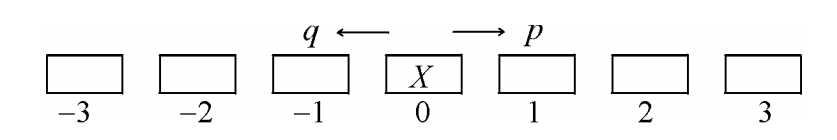
\includegraphics[width=0.86\textwidth]{rw.png}
  


 Let $X_0=0$ and  
$X_n = \sum_{i=1}^n Z_i$, 
where the iid random variable $Z_i$ is defined as follows
\[
Z_i = \begin{cases}
 +1,  \quad \mbox{with prob } p= 0.5 \\
 -1,  \quad \mbox{with prob  } 1-p=0.5 \\
\end{cases}
\]
The case of $p=q=1/2$ is called symmetric random walk.

}


\frame{ {The random walk is a DTMC on $S=\ZZ$ }

Proof of Markovian property:
\pause
\[
\begin{split}
&\p(X_{n+1}=j \vert X_{n}=i, X_{n-1}, \cdots, X_{0} )\\
=&\p(X_{n}+Z_{n+1}=j \vert X_{n}=i, X_{n-1}, \cdots, X_{0}  )\\
=&\p(Z_{n+1} = j-X_{n}\vert X_{n}=i, X_{n-1}, \cdots, X_{0} )\\
=&\p(Z_{n+1} = j-i\vert X_{n}=i  )   ~~\because {\small Z_{n+1}\mbox{ indpt. of } \{X_n, X_{n-1}, \ldots\}}
\\
=&\begin{cases}
p & \mbox{ if } j=i+1;\\
q & \mbox{ if } j=i-1;\\
0 & \mbox{ else}.
\end{cases}
\end{split}
\]


\bigskip\pause
Question:    What is the transition diagram and transition matrix ? 

\pause

\[
\Pm=\left[\begin{array}{cccccc}
\cdots & q &  0&  p&\cdots &\cdots\\
\cdots & \cdots &  q&  0&p &\cdots\\
\ddots & \ddots & \ddots & \ddots& \ddots& \ddots \\
\end{array}\right]
\]




}




\begin{frame}
\frametitle{Random Walk}
\framesubtitle{  random walk  on finite interval of $\mathbb{Z}$}

 Let $-M,N$ be two positive integers, 
define a random walk on 
\[ S = [-M,N]\cap \ZZ
=\{-M,-M+1,\cdots, N-1,N\}.
\]
The particle $X_n$ will randomly jump to one of its two neighbors, 
according to probability $p$ and $q$ where $p+q=1$.
Define 
$\p(X_{n+1}=i+1| X_n=i) = p$, $\p(X_{n+1}=i-1| X_n=i) = q$
for any {\em interior} point $i$.

\medskip
\pause

For finite interval $[-M, N]$, we need specify the boundary condition
\setbeamersize{description width=-\labelsep}

\begin{description}[<+->]
\item{1. \underline{absorbing} (gambler's ruin problem)}

$\p(\Xnn=N|\Xn=N)=1$ and 
$\p(\Xnn=-M|\Xn=-M)=1$

\item{2. \underline{reflection} (elastic wall)}

$\p(\Xnn=N-1|\Xn=N)=1$ and 
$\p(\Xnn=-M+1|\Xn=-M)=1$

\item{3. \underline{periodic} (  walk on a circle)}

$\p(\Xnn=-M|\Xn=N)=p$ and
$\p(\Xnn=N|\Xn=-M)=q$


\end{description}


\end{frame}

\frame{
\bizp
\item absorbing boundary condition


\[
\Pm=\left[\begin{array}{ccccc}
1 & 0 &  0&  0&0 \\
q & 0 &  p&  0&0 \\
0 & q &  0&  p&0 \\
0 & 0 & q&  0&p \\
0 & 0 &  0&  0&1 \\
\end{array}\right]
\]

\item reflection boundary condition


\[
\Pm=\left[\begin{array}{ccccc}
0 & 1 &  0&  0&0 \\
q & 0 &  p&  0&0 \\
0 & q &  0&  p&0 \\
0 & 0 & q&  0&p \\
0 & 0 &  0&  1&0 \\
\end{array}\right]
\]


\item periodic boundary condition


\[
\Pm=\left[\begin{array}{ccccc}
0 & p &  0&  0&q \\
q & 0 &  p&  0&0 \\
0 & q &  0&  p&0 \\
0 & 0 & q&  0&p \\
p & 0 &  0&  q&0 \\
\end{array}\right]
\]




\eiz
}


%
%\begin{frame}
%\frametitle{Random walk}
%%
%%Physical applications:  Brownian motion (continuous version of random walk),
%%diffusion process.
%%
%%Financial application:  binomial tree model. $X_n$ correspond to  logarithm  of return at time $n$. 
%%
%  
%
%We shall answer the following questions
%\begin{itemize}
%\item  expected value of $X_n$,  $\e(X_n)$
%\item What is the behavior of the distribution of $X_n$ as $n\to\infty$ ?
%\item  the expectation of the first hitting time    $\inf \left \{n: \p(X_n) = x)\right \}  $
%\item  probability of hitting left boundary point before 
%hitting the right  boundary point for absorbing boundary conditon
%$$\p(X_\tau=-M)$$ where $\tau=\inf\{n: X_n \in \{-M, N\}\}$
%is the first exit time.
% 
%\end{itemize}
%
%\end{frame}
%
%\begin{frame}
%\frametitle{Reading Assignment: Examples of Markov Chain}
%
%{\bf Read example 2.2-2.7, page 8-13\footnote{
%This number refers to the textbook:
%Introduction to
%Modeling and Analysis of Stochastic Systems. (Second Edition)
%}
%}
%
%
%Pay attention to these points:
%
%\begin{itemize}
%\item  Modeling: Formulate the real problem in probability language.
%\begin{itemize}
%\item
%How to define random variables at each time  (\ie, stochastic process)?  continuous time or discrete time?
%\item What is the state space ?  Is it discrete or continuous ? 
%\item How to express the output of interest using the stochastic process you have set up ? 
%\end{itemize}
%\item  Markov Model
%\begin{itemize}
%
%\item Is the  Markovian assumption reasonable?
%\item Is it time homogeneous \MC? 
%\item Write down the \tm and transition diagram.
%\end{itemize}
%
%
%\end{itemize}
%
% 
%  
% \end{frame}

\frame{{Random Walk on Graph}
Consider a connected graph  without self-loop with node $S=\set{1,2,\ldots,N}$.
The walker at state $i$ goes to one of its direct neighbours with equal probability
$1/d_i$, where $d_i$ is the degree of node $i$.
For undirected graph, the movement direction is bi-directional. 
\begin{center}
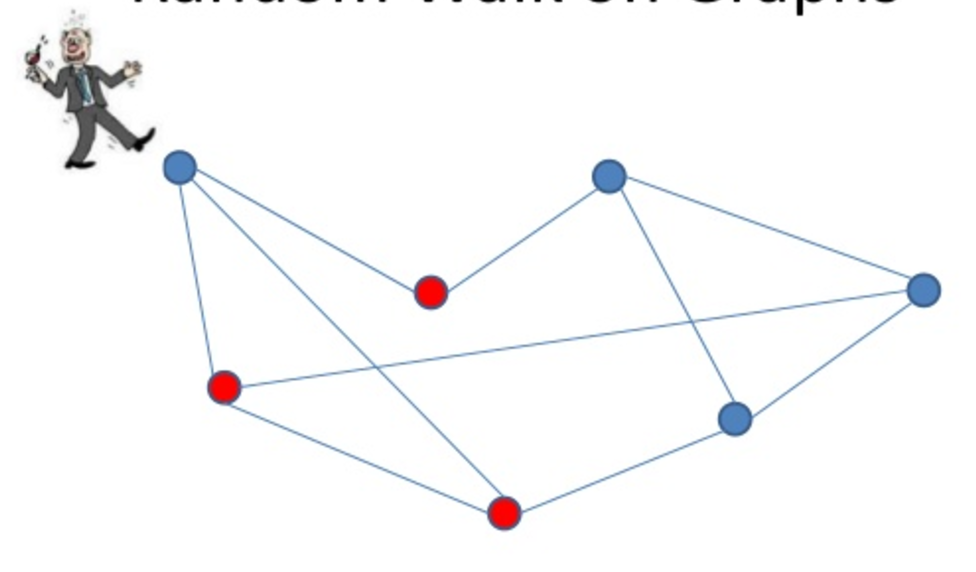
\includegraphics[scale=0.26]{rwog.png}
%/includegraphics[scale=0.1]{twitter_network.jpg}
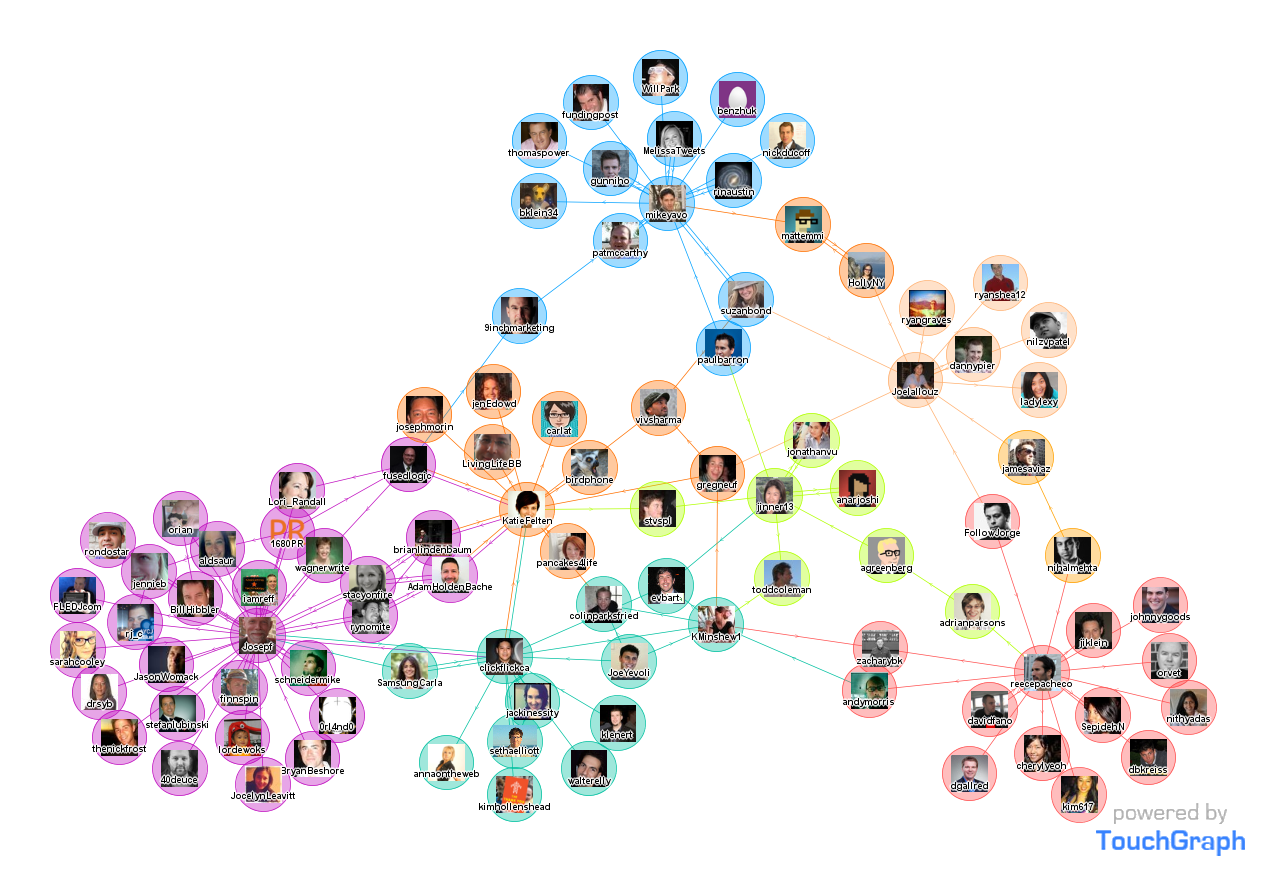
\includegraphics[scale=0.14]{TouchGraph.png}
\end{center}
}

\begin{frame}
{\Large Transient Distribution: $\p(X_n=j)=?$}

For the symmetric random walk,  we worked very  hard to obtain if $X_0=0$, then

\[ \p(X_1=1)=p,  \p(X_1=-1)=q,
\]
\[ \p(X_2=2)=p^2,  \p(X_2=0)=2pq,  \p(X_2=-2)=q^2,
\]
\[  
  \p(X_3=3)=p^3,  \p(X_3=1)=3p^2q,      
  \p(X_3=-1)=3pq^2,
  \p(X_3=-3)=q^3, 
\]
\[\cdots\]
\end{frame}



\begin{frame}
{  there is an easy way to calculate for DTMC }
\framesubtitle{you need know matrix-vector multiplication and matrix power.}


\biz[<+->]
\item Let the state space $S=\{1,2,\ldots, N\}$. Specify  an initial distribution at time $t=0$: $\p(X_0=j)=a_j$
where $a=(a_1,a_2,\cdots,a_N)$ satisfies $a_j\geq 0 \ \forall j$ and $\sum_{j=1}^N a_j=1$.
(called a {\it stochastic vector}  or {\it probability vector}.)
\item 
Define $n$-step transition probability in matrix form $\Pm^{(n)}=[p^{(n)}_{ij}]$:  
\[ p^{(n)}_{ij} \triangleq \p(X_n=j|X_0=i),
 ~~ \Pm^{(0)}=\eye,  ~~\Pm^{(1)}=\Pm.\]
  
\item From Law of Total Probability, for any $j\in S$,
\begin{equation}\label{eqn:Xn}
\p(X_n=j)=  \sum_{i\in S} \p(X_n=j|X_0=i) \p (X_0=i)= \sum_i p^{(n)}_{ij} a_i = (a\Pm^{(n)})_j
\end{equation}
here $a\Pm^{(n)}$ is a (row)vector-matrix multiplication. 
\eiz
\end{frame}



\frame{
{Joint distribution (path distribution)
}
What is the probability that 
the sample path of the (time homogeneous) DTMC 
is $(X_0,X_1,X_2,\cdots, X_n) = (i_0,i_1,i_2, \cdots, i_n)$?
i.e., the joint distribution of  $(X_0,X_1,X_2,\cdots, X_n) $?
\pause
%Denote $a^{(0)}$   the initial distribution of $X_0$ and $\Pm=[p_{ij}]$
%the transition matrix.
\begin{equation}\label{eqn:X1n}
\tag{$\triangle$}
\begin{split}
&\p \bigg(  (X_0,X_1,X_2,\cdots, X_n) = (i_0,i_1,i_2, \cdots, i_n)  \bigg)
\\
= & \p(X_0=i_0) \times \p( X_1=i_1,X_2=i_2,\cdots, X_n= i_n \mid X_0=i_0) 
\\
=& a _{i_0}
\p( X_1=i_1 \mid X_0=i_0)
 \times \p( X_1=i_1,X_2=i_2,\cdots, X_n= i_n \mid X_0=i_0, X_1=i_1) 
\\=& a _{i_0} p_{i_0,i_1}  \p(  X_2=i_2,\cdots, X_n= i_n \mid X_1=i_1) 
\\ = & 
\cdots
\\
=& a _{i_0} \times p_{i_0,i_1} \times  p_{i_1,i_2} \times p_{i_{n-1},i_n}
\end{split}
\end{equation}
So, the marginal distribution for $X_n$ is 

\pause
\begin{equation}\label{eqn:Xnj}
\p(X_n=i_n) = 
\footnote{In the continuous limit (diffusion),
these ``sums'' become the so-called {\it path-integral}. }
\sum_{i_0}\sum_{i_1}\cdots \sum_{i_{n-1}} \eqref{eqn:X1n}
=
(a   \Pm ^n)_{i_n}
\end{equation}
\pause
Compare \eqref{eqn:Xn} and \eqref{eqn:Xnj} which hold for any vector $a$,
then 
\[ a\Pm^{(n)} = a\Pm^n \Longrightarrow \Pm^{(n)} = \Pm^n .\]
}


\frame{
{$n$-step transition matrix}
\begin{theorem}[ (for time-homogeneous MC). Thm 2.2]
\[\Pm^{(n)} = \Pm^n.\]
where $\Pm^{n}$ is the nth power of the one-step transition matrix $\Pm$.
\end{theorem}
\pause
\bigskip 
We also  have the following important property due to time homogeneity (invariant under time shift)
\begin{block}{(Cor. 2.2)}
\[ \p(X_{n+k}=j|X_k=i)   = \p(X_n=j|X_0=i)  = p^{(n)}_{ij}  , \forall k
\]
\end{block}


}

\frame{Properties of transition matrix}

\begin{frame}
\begin{definition}
An $N\times N$ matrix $P=[p_{ij}]$ is called a stochastic matrix if 
\begin{enumerate}[<+->]
\item $p_{ij\geq0}$ for all $i,j$.
\item $\sum_{j=1}^{N}p_{ij}=1$ for all $i$.  That is  the sum of each row is
$1$. In matrix form, $P\onem=\onem$, where $\onem=(1,1,\cdots,1)^\tr$
\end{enumerate}
\end{definition}
\pause
$\lambda_1=1$ is one of the eigenvalues of any stochastic matrix.
\pause
\begin{theorem}
\bizp
\item
The transition matrix $\Pm$ is a stochastic matrix.
\item 
  $\Pm^n$ for any integer  $n\geq 0$ is a stochastic matrix.
  \eiz
\end{theorem}
\pause
Furthermore, $\Pm$  satisfies (\optional)
\biz[<+->]
\item All eigenvalues (complex value possibly ) satisfy $|\lambda_i|\leq 1$ (Perron-Frobenius theorem). So, the spectral radius  
\[ \rho(\Pm)\triangleq \max_i |\lambda| =1.\]
\item {\it $\lambda_1=1$ might not be the only eigenvalue on the unit circle and the associated eigenspace can be multi-dimensional.}
\eiz

\end{frame}

\begin{frame}
\frametitle{Chapman\textendash{}Kolmogorov Equation}

This is the most fundamental equation for Markov process (not limited to time-homogeneous case,
even not to the discrete time or discrete state space).

\bigskip 
\begin{theorem}[Thm 2.3]
The n-step transition probabilities $\Pm^{(n)}$ satisfy the following equation,
called the Chapman\textendash{}Kolmogorov equation:

\[
p_{ij}^{(n+m)}=\sum_{k=1}^{N}p_{ik}^{(n)}p_{kj}^{(m)}.
\]
\end{theorem}%{}

Remark :  For time homogeneous DTMC, this is the simple fact for any square matrix $\Pm$:
$\Pm^{n+m}=\Pm^{n}\Pm^{m}$

{\it Proof}: textbook page 18.
\end{frame}

\frame{Occupancy Times}

\frame{
{\bf Occupancy time} is  the expected amount of time
that the  Markov chain spends in a given state during a given interval of time.

\begin{block}{Occupancy Times}
\biz[<+->]
\item Let $N_j^{(n)}$ be the number of times the DTMC visits state $j$ over the time span $\{0,1,2,\cdots,n\}$.
That is 
 $N_j^{(n)}=\sum_{t=0}^n 1_{\{X_t=j\}} $, where  $1_{\{\cdot\}}$ is the indicator function.
\item  $m_{i,j}^{(n)}=\e (N_j^{(n)}|X_0=i)$ is the occupancy time up to $n$ of state $j$ starting from
state $i$.
\item occupancy times matrix: $\Mm^{(n)} = [m_{i,j}^{(n)}] $.
\eiz
\end{block}
}

\frame
{
\begin{theorem}[Thm 2.4]
\[ \Mm^{(n)} = \sum_{t=0}^n \Pm^t.\]
\end{theorem}
Occupancy time is the sum of all $t$-step transition matrices.

\medskip
{\it Proof} : see textbook page 22.
(or see next slide for proof of a general case.)

}




\begin{frame}
\frametitle{Generalization:   Cost Models over a finite time \footnote{Section $2.6.1$}}

Let $c(x): S \to \Real$ be a cost function. The expectation of the total cost up to time $n$ is 
\[ C_i^{(n)} \triangleq \e \left[\sum_{t=0}^n c(X_t)\vert X_0=i\right]. \]
For a general $c(x)$,  the calculation    is below  (Theorem 2.11 (page 35)).
\[
\begin{split}
C_i^{(n)} &=\sum_{t=0}^n   \e \left[ c(X_t) (\sum_{j\in S} 1_{\set{X_t =j}}) \mid X_0=i\right] (\because\mbox{ law of total prob.})\\
&=\sum_{t=0}^n \sum_{j\in S} \e \left[ c(X_t)
\mid X_t=j, X_0=i\right]\p \left( X_t = j    \mid X_0=i\right) (\because\mbox{ cond. prob.})\\
&=\sum_{t=0}^n \sum_{j\in S} c(j)p^{(t)}_{ij} = 
\sum_{j\in S} c(j) \sum_{t=0}^n p^{(t)}_{ij} 
\end{split}
\]
\pause
The equivalent matrix-vector multiplication form is 
($c=(c(1),c(2),\cdots,c(N))^\tr$ is column vector )
 \begin{equation} \label{C}
 \boxed{
  C^{(n)} = \left ( \sum_{t=0}^n \Pm^t \right ) c}
  \end{equation}

\end{frame}


\frame{

 In particular, if $c(\cdot): S \to \Real$ is the indicator function $1_{\set{j}}(\cdot)$, then
 by definition,
\[ C_i^{(n)} = \e \left[\sum_{t=0}^n 1_j (X_t)\vert X_0=i\right]
 = \e \left[ N^{(n)}_j \vert X_0=i\right]=m_{i,j}^{(n)}
 \]
which is  the occupancy time of state $j$.
On the other hand, the previous slide told us that
the above line is actually equal to 
\[ 
\sum_{j' \in S} c(j') \sum_{t=0}^n p^{(t)}_{ij'} =
\sum_{j' \in S}  1_{\set{j}}(j') \sum_{t=0}^n p^{(t)}_{ij'}  =  \sum_{t=0}^n p^{(t)}_{ij} 
\]

So, we have shown  [Thm 2.4]:
\[ \Mm^{(n)} = \sum_{t=0}^n \Pm^t.\]

Then   \eqref{C} can be written in terms of $\Mm^{(n)}$:
 \[\boxed{ C^{(n)} = \Mm^{(n)}  c}\]

}

\frame{{\hw}

\biz

\item  Let $X_n$  be the random walk on $S=\ZZ$ with transition probability
$\p(X_{n+1}=i+1\vert X_n) = p$
and $\p(X_{n+1}=i-1\vert X_n) = q=1-p$.

Calculate the mean $\e X_n$, the variance $\Var{X_n}$
and the autocovariance 
$\e[(X_n - \e X_n)(X_m - \e X_m)]$.
%answer 0, 4pq, \min(n,m)4pq.

  
\item  
 Assume that $\{X_n\}$, $n=0,1,2,\cdots,$ are iid  $\{-1,1\}$-valued random variables.
 $\p(X_i=1)=p$ and $\p(X_i=-1)=1-p$.   
For any $n\geq 1$,  define new random variables 
 \[ 
 S_n \triangleq \sum_{i=0}^n X_i, \
   Y_n\triangleq  X_{n}+X_{n-1}, 
 \]
   and the   two-dim random vector
   $
        Z_n\triangleq \begin{bmatrix} X_{n-1} \\ X_n\end{bmatrix}
   $.
Discuss if  the  stochastic processes $\{S_n\}$,  $\{Y_n\}$,  $\{Z_n\}$, are Markov chains.
Why? 
Write the corresponding transition matrices  for Markov chains.
 \item textbook page 51:  2.13, 2.16\\
\item textbook page 53-54: 2.10, 2.11, 2.15(b).
\footnote{MATLAB  command for power of  a matrix is : {$\mathrm {A\, \hat{ }\, n}$}.}

\eiz

}


\end{document}
